\documentclass[10pt,a4paper]{article}
\usepackage[utf8]{inputenc}
\usepackage[T1]{fontenc}
\usepackage[french]{babel}
\usepackage{lmodern,microtype}
\usepackage[margin=1.85cm,top=1.7cm,bottom=1.8cm]{geometry}
\usepackage{amsmath,amssymb}
\usepackage{graphicx,float,caption}
\usepackage[hidelinks]{hyperref}
\usepackage{fancyhdr}
\usepackage{enumitem}
\setlist[itemize]{nosep,leftmargin=1.4em}
\setlength{\parindent}{0pt}
\setlength{\parskip}{4pt}
\setlength{\headheight}{13pt}
\pagestyle{fancy}\fancyhf{}
\lhead{Master 2 Informatique -- VMI}
\rhead{Reconnaissance de formes avancée}
\cfoot{\thepage}
\graphicspath{{figures/}{../}}
\newcommand{\norm}[1]{\left\lVert #1\right\rVert}
\title{\vspace{-1.3cm}\textbf{TP -- Fuzzy C-means}\\[0.25em]\large Segmentation d'image en régions floues}
\author{Roméo Agostino}
\date{}
\begin{document}
\maketitle
\vspace{-1.0cm}
\begin{center}
Code source : \url{https://github.com/RomeoAg13/Fuzzy-image-clustering}
\end{center}

\section{Introduction}
La segmentation consiste à regrouper les pixels d'une image selon leurs caractéristiques. Contrairement à une segmentation dure, qui affecte chaque pixel à une seule classe, la segmentation floue associe à chaque pixel plusieurs degrés d'appartenance. Le but de ce TP est d'implémenter l'algorithme Fuzzy C-means (FCM), puis d'appliquer cet algorithme à la segmentation d'une image en régions floues avec des images à niveaux de gris. Le résultat est visualisé avec une heatmap.

\section{Principe du Fuzzy C-means}
On considère $N$ pixels $X=\{x_1,\ldots,x_N\}$, $C$ clusters et un coefficient de flou $m>1$. \\ La matrice $U=(u_{ij})\in[0,1]^{N\times C}$ décrit l'appartenance du pixel $i$ au cluster $j$. \\ Pour chaque pixel, $\sum_{j=1}^{C}u_{ij}=1$. L'algorithme minimise la fonction objectif :
\begin{equation*}
J_m(U,c)=\sum_{i=1}^{N}\sum_{j=1}^{C}u_{ij}^{m}\norm{x_i-c_j}^{2}.
\end{equation*}
Les centres $c_j$ sont les moyennes pondérées des valeurs des pixels, et les appartenances sont recalculées à partir de leurs distances aux centres :
\begin{align*}
c_j&=\frac{\sum_{i=1}^{N}u_{ij}^{m}x_i}{\sum_{i=1}^{N}u_{ij}^{m}}, \\[2pt]
u_{ij}&=\left[\sum_{k=1}^{C}\left(\frac{\norm{x_i-c_j}}{\norm{x_i-c_k}}\right)^{\frac{2}{m-1}}\right]^{-1}.
\end{align*}
La formule d'appartenance suppose des distances non nulles dans les dénominateurs, les distances nulles sont traitées séparément dans le programme. Pour $C=2$, avec $d_1=|x_i-c_1|$ et $d_2=|x_i-c_2|$ non nuls, la mise à jour utilisée est :
\begin{equation*}
u_{i1}=\frac{1}{1+(d_1/d_2)^{2/(m-1)}},\qquad u_{i2}=1-u_{i1}.
\end{equation*}

\section{Implémentation et protocole expérimental}
L'implémentation Python est organisée en cinq fonctions :
\begin{itemize}
  \item \texttt{create\_membership\_matrix} qui initialise $U$
  \item \texttt{calculate\_centroids} qui calcule les centres 
  \item \texttt{update\_matrix} qui actualise les appartenances
  \item \texttt{stop\_criteria} qui mesure leur variation maximale
  \item \texttt{fuzzy\_c\_means} qui répète ces étapes jusqu'à convergence ou jusqu'à la limite d'itérations.
\end{itemize}
Les paramètres utilisés sont $C=2$, $m=2$, $\varepsilon=0{,}01$ et $T_{\max}=100$.

À chaque itération $t$, les centres puis les appartenances sont recalculés. L'algorithme s'arrête lorsque la plus grande variation d'un degré d'appartenance passe sous le seuil $\varepsilon$ :
\begin{equation*}
\max_{i,j}\left|u_{ij}^{(t)}-u_{ij}^{(t-1)}\right|<\varepsilon,
\end{equation*}
ou lorsque le nombre d'itérations atteint $T_{\max}$.

Le protocole expérimental est le suivant :
\begin{itemize}
  \item L'image \texttt{milky-way-nvg.jpg} fournie pour le TP est en niveaux de gris et mesure initialement $1024\times1024$ pixels.
  \item Elle est redimensionnée en $128\times128$ pixels afin de réduire le temps de calcul.
  \item Après conversion en tableau NumPy, \texttt{flatten()} produit un vecteur de $16\,384$ intensités.
  \item FCM retourne $U$ de forme $(16\,384,2)$, \texttt{reshape(128,128,2)} permet de retrouver deux cartes spatiales des appartenances, une par cluster.
\end{itemize}

\section{Résultats et discussion}
\begin{figure}[H]
\centering
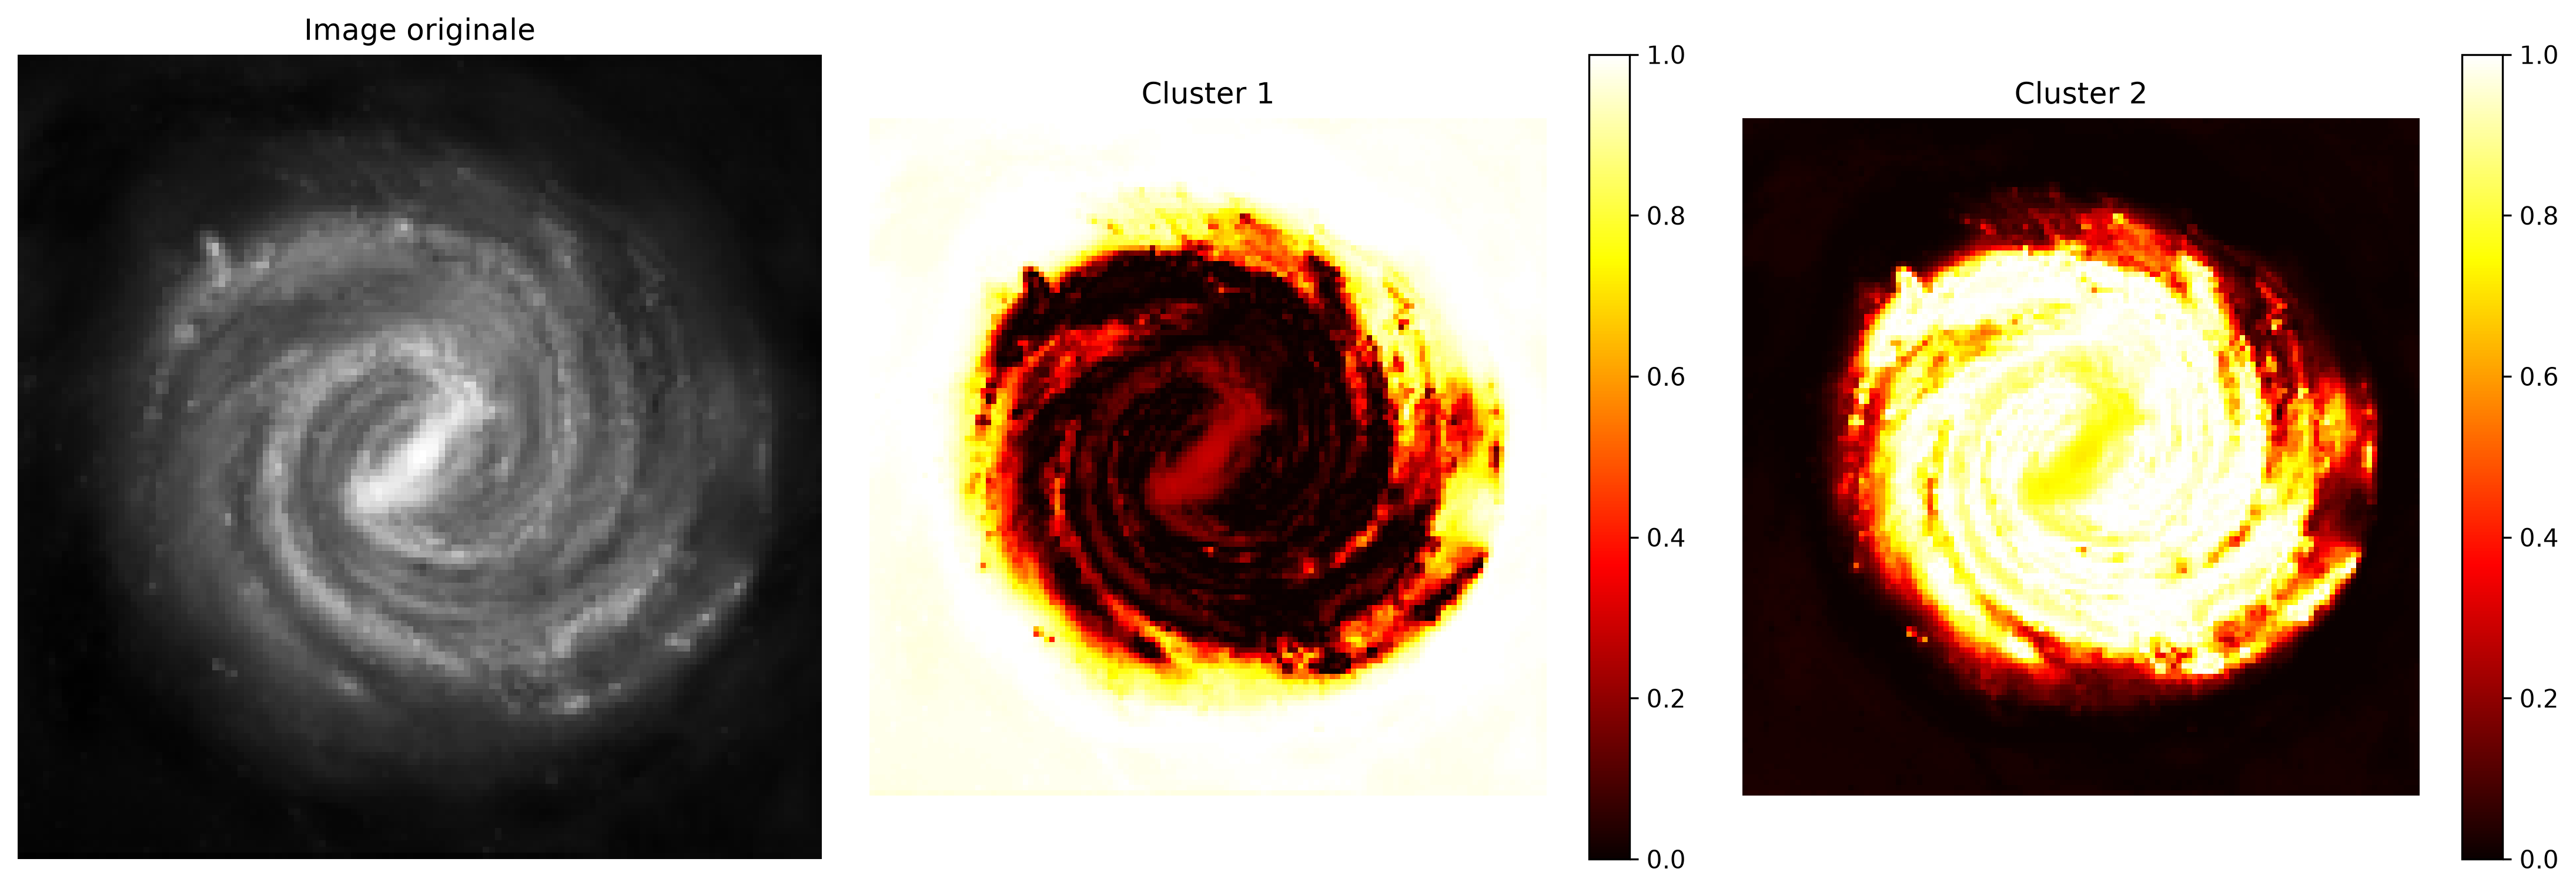
\includegraphics[width=\textwidth]{segmentation_fcm_grayscale.png}
\caption{Image de la galaxie en niveaux de gris et cartes de chaleur des degrés d'appartenance aux deux clusters. Une valeur claire indique une forte appartenance.}
\label{fig:resultats}
\end{figure}

La figure 1 montre que le regroupement distingue principalement le fond sombre des structures plus lumineuses de la galaxie (noyau et bras spiraux). Les deux cartes sont complémentaires puisque $u_{i1}+u_{i2}=1$ pour chaque pixel. Lors d'une exécution, les centres étaient proches de $27{,}25$ et $111{,}49$ niveaux de gris

FCM segmente uniquement selon l'intensité, sans tenir compte des pixels voisins : chaque pixel est réduit à sa valeur de gris avant le calcul, et sa position dans l'image n'intervient pas. Deux pixels de même intensité reçoivent donc les mêmes degrés d'appartenance, même s'ils sont éloignés. Aucune cohérence spatiale n'est imposée aux régions obtenues.

Sur dix exécutions avec des initialisations différentes, l'algorithme a convergé en 9 à 12 itérations, bien avant la limite $T_{\max}=100$. Les centres obtenus sont restés stables, entre $27{,}2$ et $27{,}3$ pour le premier et entre $111{,}5$ et $111{,}6$ pour le second.

\end{document}